\begin{figure}[!ht]
 \centering
 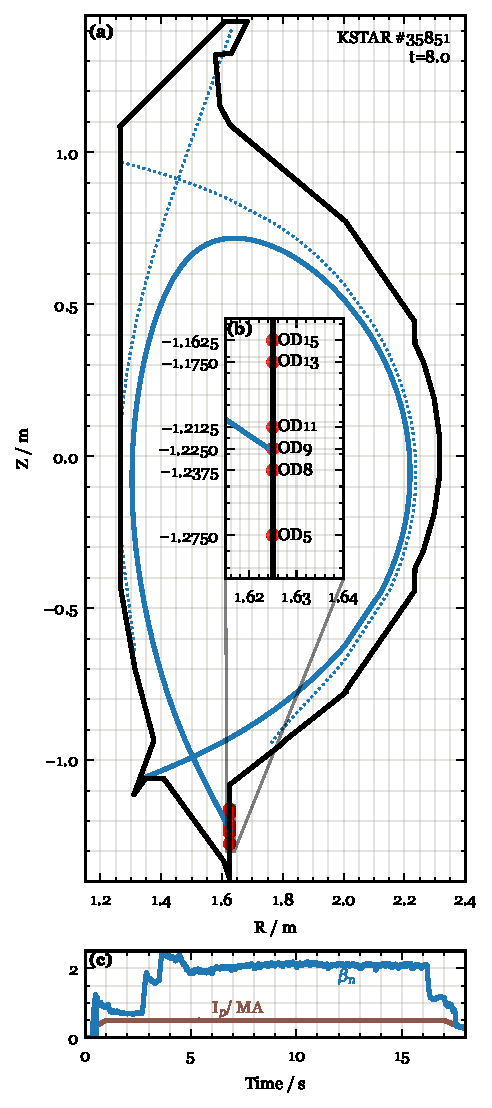
\includegraphics[width=\linewidth]{figures/RefShot_35851.pdf}
 \caption{
Reference shot \#35851.
(a) Showing last closed flux surface at t=8 seconds.
The magnetic shape control was programmed to keep X point fixed which provided a sufficiently stable strike point on the realtime Langmuir Probe array.
(b) Zoomed-in locations of realtime Outer Divertor (OD) Langmuir probes.
(c) Plasma current (I$_p$) and $\beta_n$ for reference shot.
}
 \label{fig:ref_shot}
\end{figure}
% Consider adding a contour for the secondary separatrix (I typically have to guess and check psi_N values until I find the one that makes another X). The modelers usually like this. If you decide to include this, make the secondary contour a lighter weight than the primary.
% It may be of some minor interest to include a thin or dashed outline of the former carbon limiting surface, which I think would be purely outboard of the tungsten surface and therefore not too confusing. However, this could be too busy and I'm not sure it should go in the final. Just something to think about.